%!TEX root = CAN.tex

\begin{appendix}
\section*{Appendix}
\pagestyle{plain}
\setcounter{table}{0}
\renewcommand{\thetable}{\Alph{section}\arabic{table}}
\addcontentsline{toc}{section}{Appendix}
\addtocontents{toc}{\protect\setcounter{tocdepth}{0}}

\section{Error Estimation of the TDC calibration.}
\label{appendix:calib_error}

In this appendix, a small study of the error made on the calibration from TDC to nanoseconds is done. By simple calculation, the conversion is done is the following way:
\begin{equation*}
\begin{split}
\text{T} \: \text{[ns]} & = ( \text{TDC} - \text{Ped} ) * \text{slope} \\
& = ( \text{TDC} - \text{Ped} ) * \frac{\text{A}}{(\text{Max} - \text{Ped})} \quad \text{with A = 3920 ns}
\end{split}
\end{equation*}

To avoid correlations between the slope and the pedestal, the error is obtained by differentiating w.r.t Max and Ped. The error is then obtained via:
\begin{equation*}
\partial t^2 = \left(\frac{\partial t}{\partial Ped}\right)^2 \times \sigma_{Ped}^2 + \left(\frac{\partial t}{\partial Max}\right)^2 \times \sigma_{Max}^2 + \left(\frac{\partial t}{\partial A}\right)^2 \times \sigma_{A}^2
\end{equation*}

Assuming that $\sigma_{A}$ is null, we get the following formula:
\begin{equation*}
\partial t^2 = \frac{1}{(\text{Max} - \text{Ped})^2} \left[ \left( \frac{\text{A(TDC - Max)}}{(\text{Max} - \text{Ped})} \right)^2 \times \sigma_{Ped}^2 + \left( \frac{\text{A(TDC - Ped)}}{(\text{Max} - \text{Ped})} \right)^2 \times \sigma_{Max}^2 \right]
\end{equation*}

As one can expect, the formula is symmetric and should be minimum in the middle of the ramp as long as $\sigma_{Max}$ and $\sigma_{Ped}$ are similar. On the other hand, the error will be greater on one side or the other depending on the $\sigma$ being the biggest. The errors estimations $\sigma_{Max}$ and $\sigma_{Ped}$ are described in subsection \ref{subsec:slope_calib}. Distributions of the errors extracted can be seen in figures \ref{fig:error_ped} and \ref{fig:error_max}. Theses errors are obtained arbitrary due to the threshold and maximum variation and are likely to be over-estimated as they are not reflected in the final timing distribution. Moreover, the shift of the distribution to zero is correcting any error made on the pedestal for each channels thus $\sigma_{Ped}$ is likely very small.

\begin{figure}[htbp]
	\subfigure[Errors extracted from the edge detection for the pedestal for each chip. channel, memory-cell and BXID.\label{fig:error_ped}] {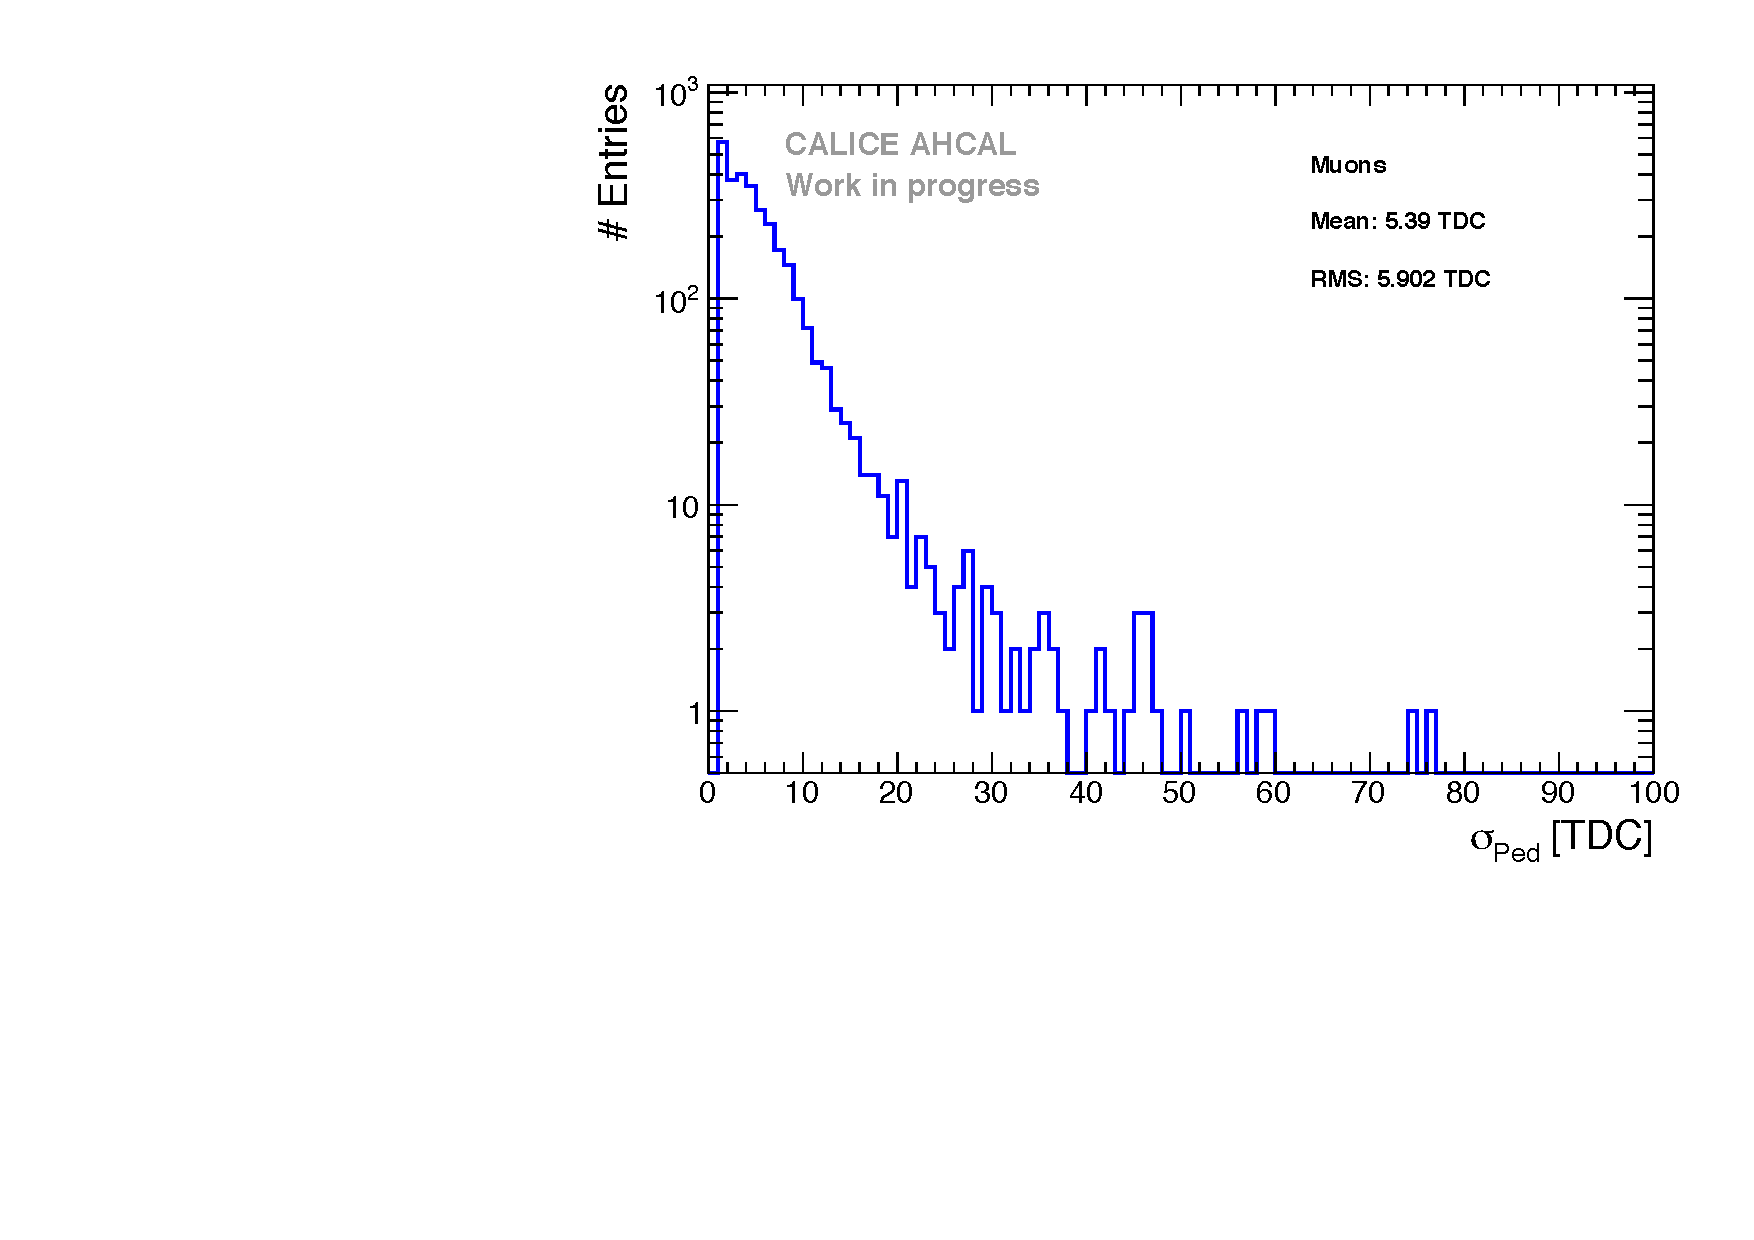
\includegraphics[width=0.5\textwidth]{fig/Muons/PedestalErrorDistribution_AHCAL.pdf}}\hfill
	\subfigure[Error extracted from the edge detection for the maximum of the ramp for each chip and BXID.\label{fig:error_max}] {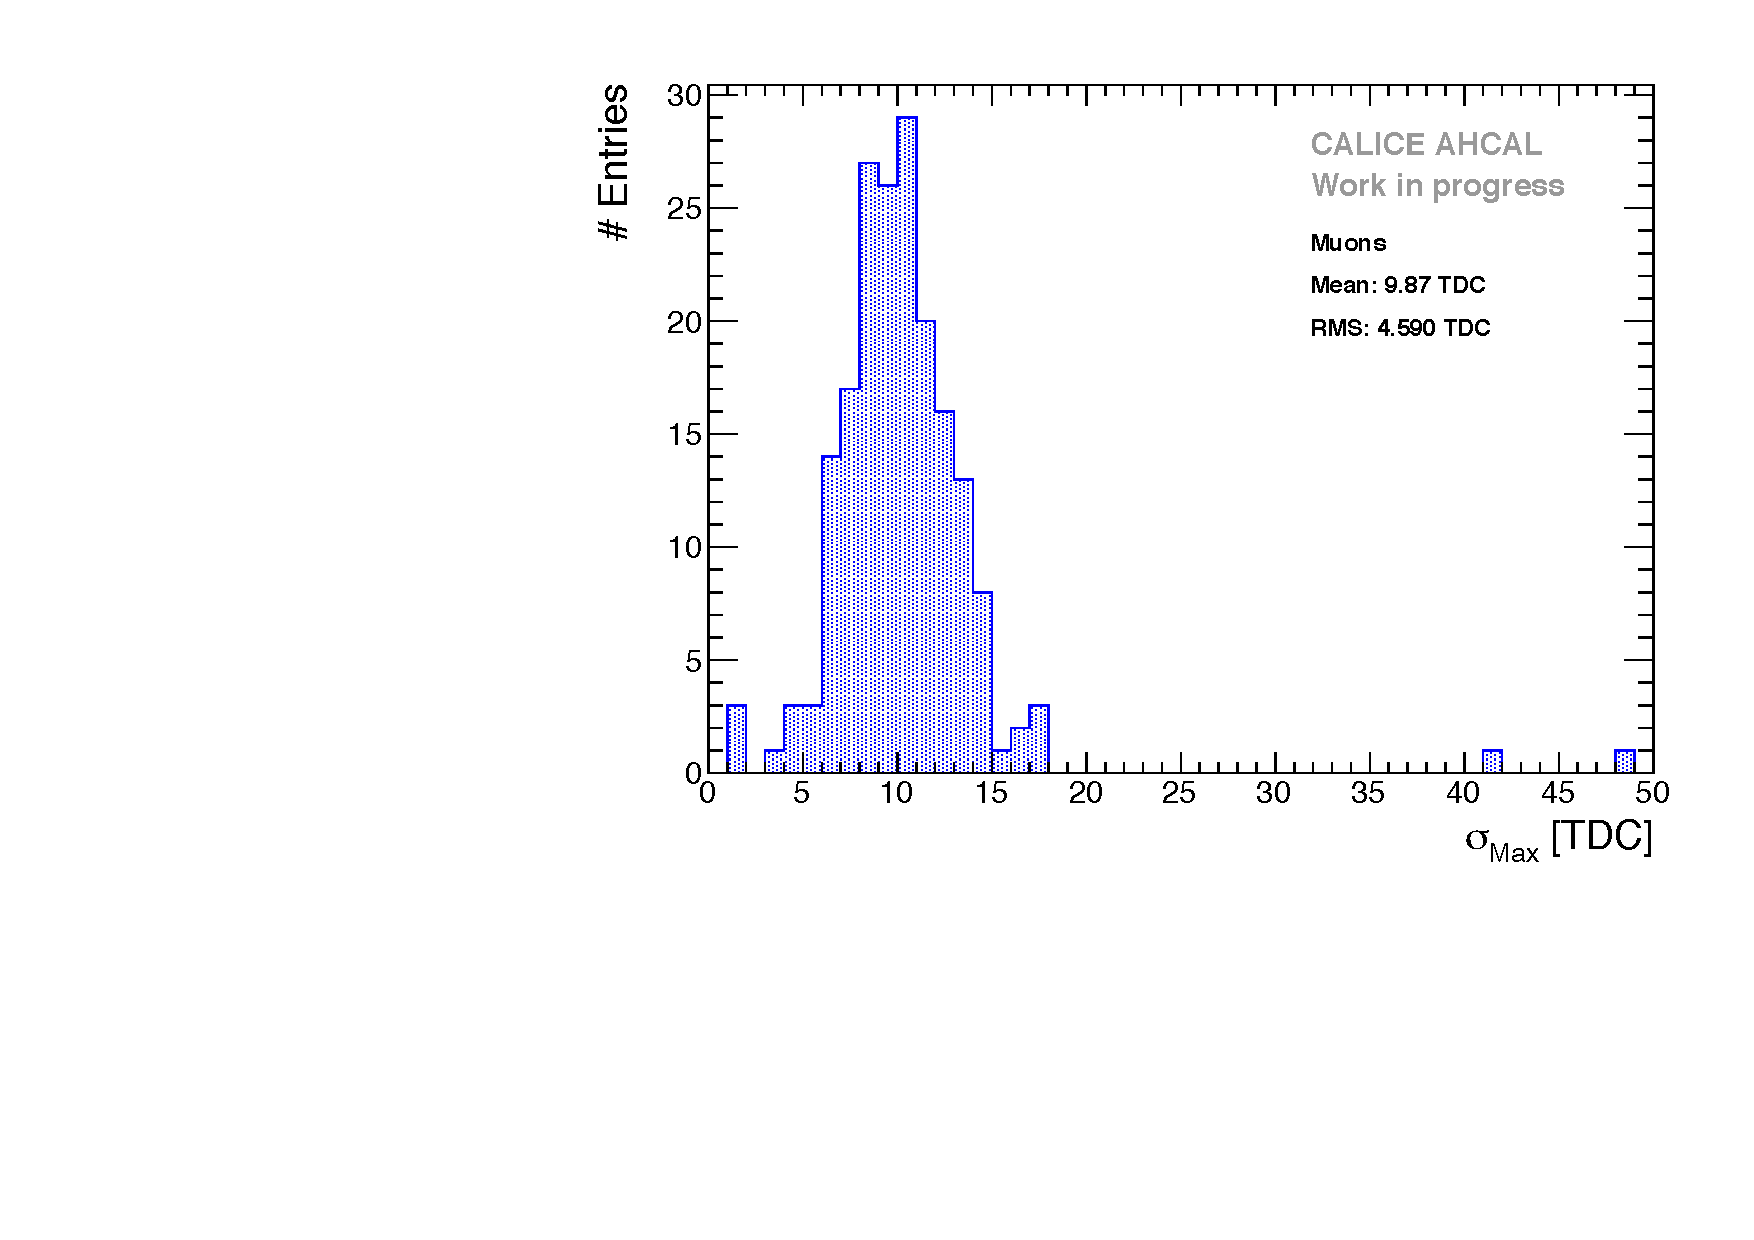
\includegraphics[width=0.5\textwidth]{fig/Muons/MaxErrorDistribution_AHCAL.pdf}}
	\caption[]{\textbf{a}: Pedestal error distribution extracted for all channels in the detector, most of the errors made are small with a high tail certainly due to the limited statistics for some channels. $\mu$ = 5.37 TDC, RMS = 5.82 TDC \textbf{b}: Maximum error distribution extracted from the edge detection method for each chip and BXID. The error is a bit higher than for the pedestal in general due to the difficulty to detect perfectly the end of the ramp. $\mu$ = 9.85 TDC, RMS = 4.60 TDC.}
	\label{fig:error_dist}
\end{figure}

The figure \ref{fig:error_chn2} represent the error made for one channel selected in a single chip for a single memory cell and BXID. It shows the symmetric behaviour of the error and present a minimum around the middle of the ramp. This not a typical channel as mostly the maximum has an error higher than the pedestal due to the difficulty to pick perfectly the maximum of the ramp with the sharp falling edge. A more typical channel can be seen in figure \ref{fig:error_chn}.

\begin{figure}[htbp]
	\subfigure[Calibration error made on the conversion to nanosecond for a channel on layer 3.\label{fig:error_chn}] {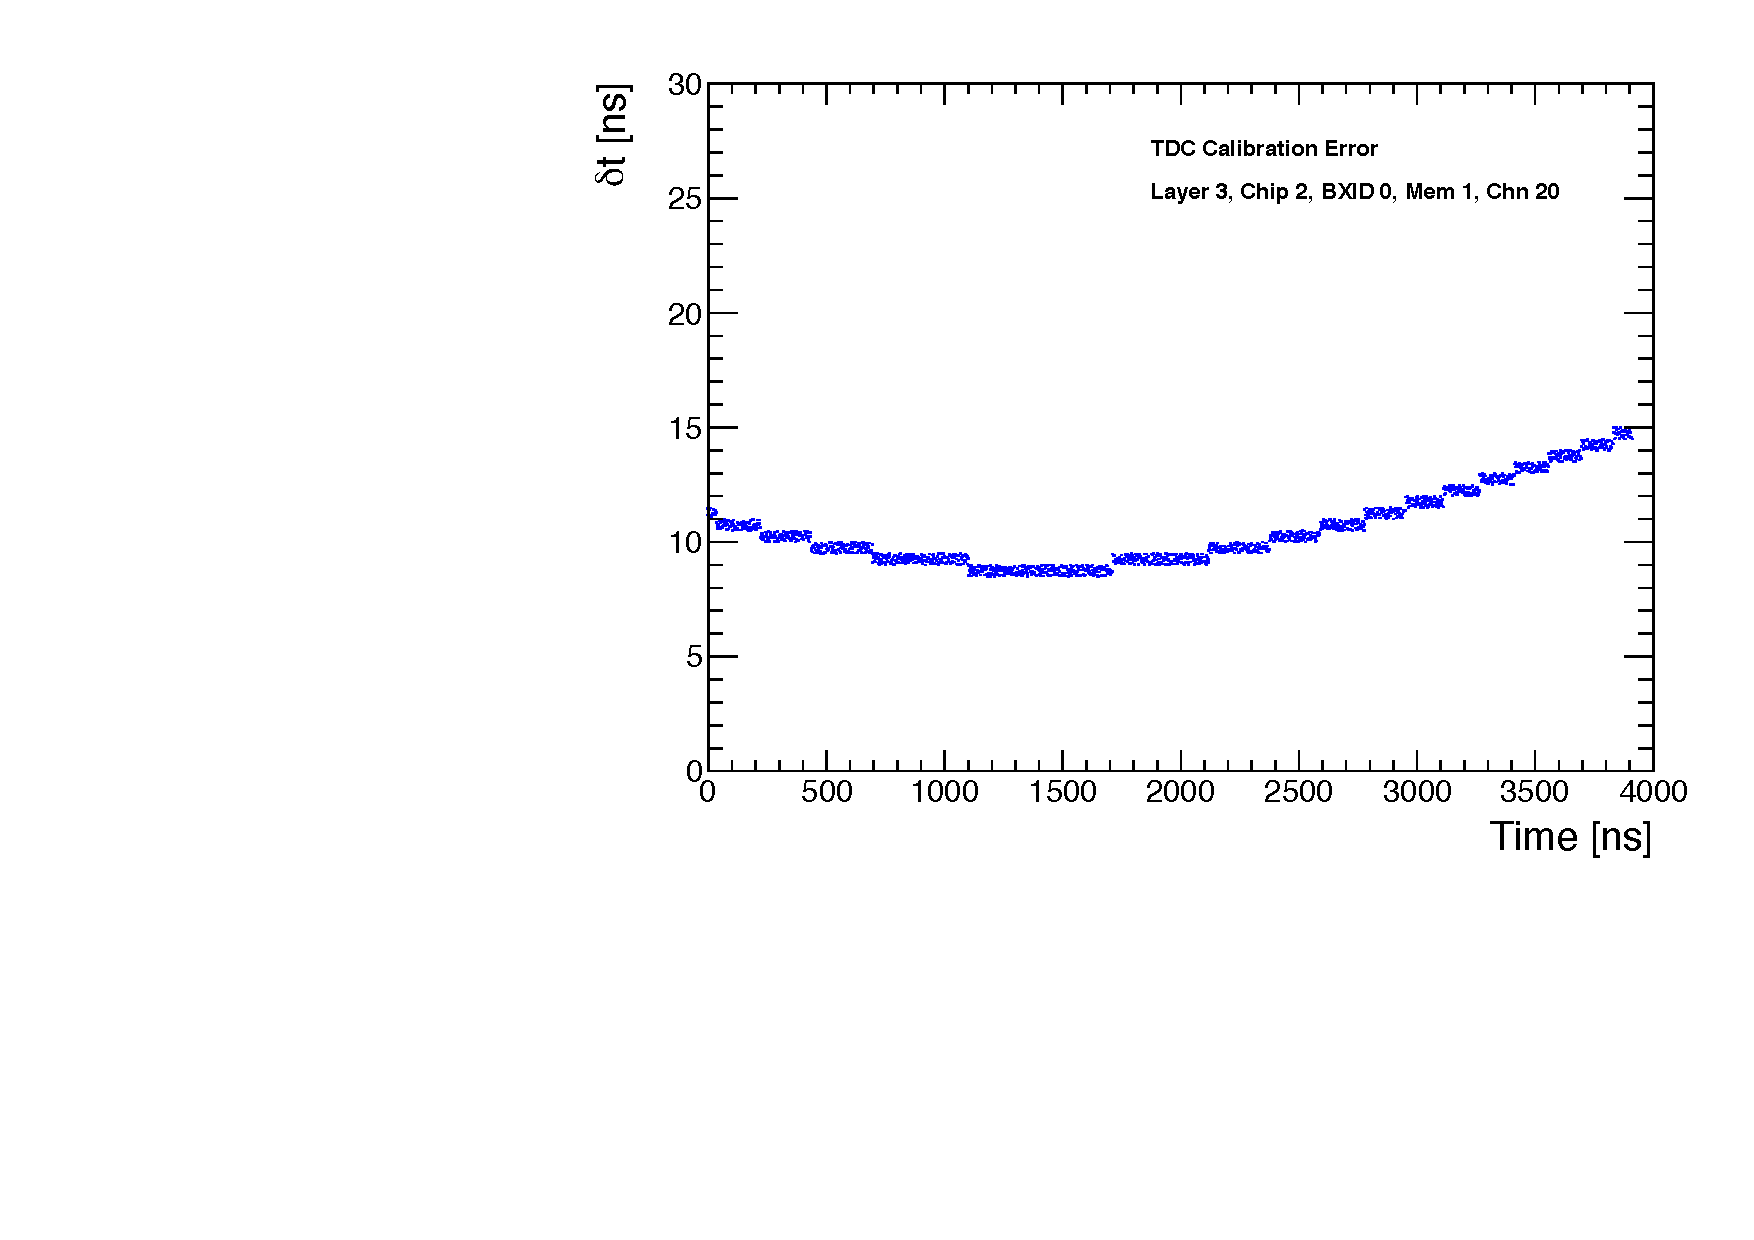
\includegraphics[width=0.5\textwidth]{fig/Muons/TimeErrorEstimation_Layer3.pdf}}\hfill
	\subfigure[Calibration error made on the conversion to nanosecond for a channel on layer 5.\label{fig:error_chn2}] {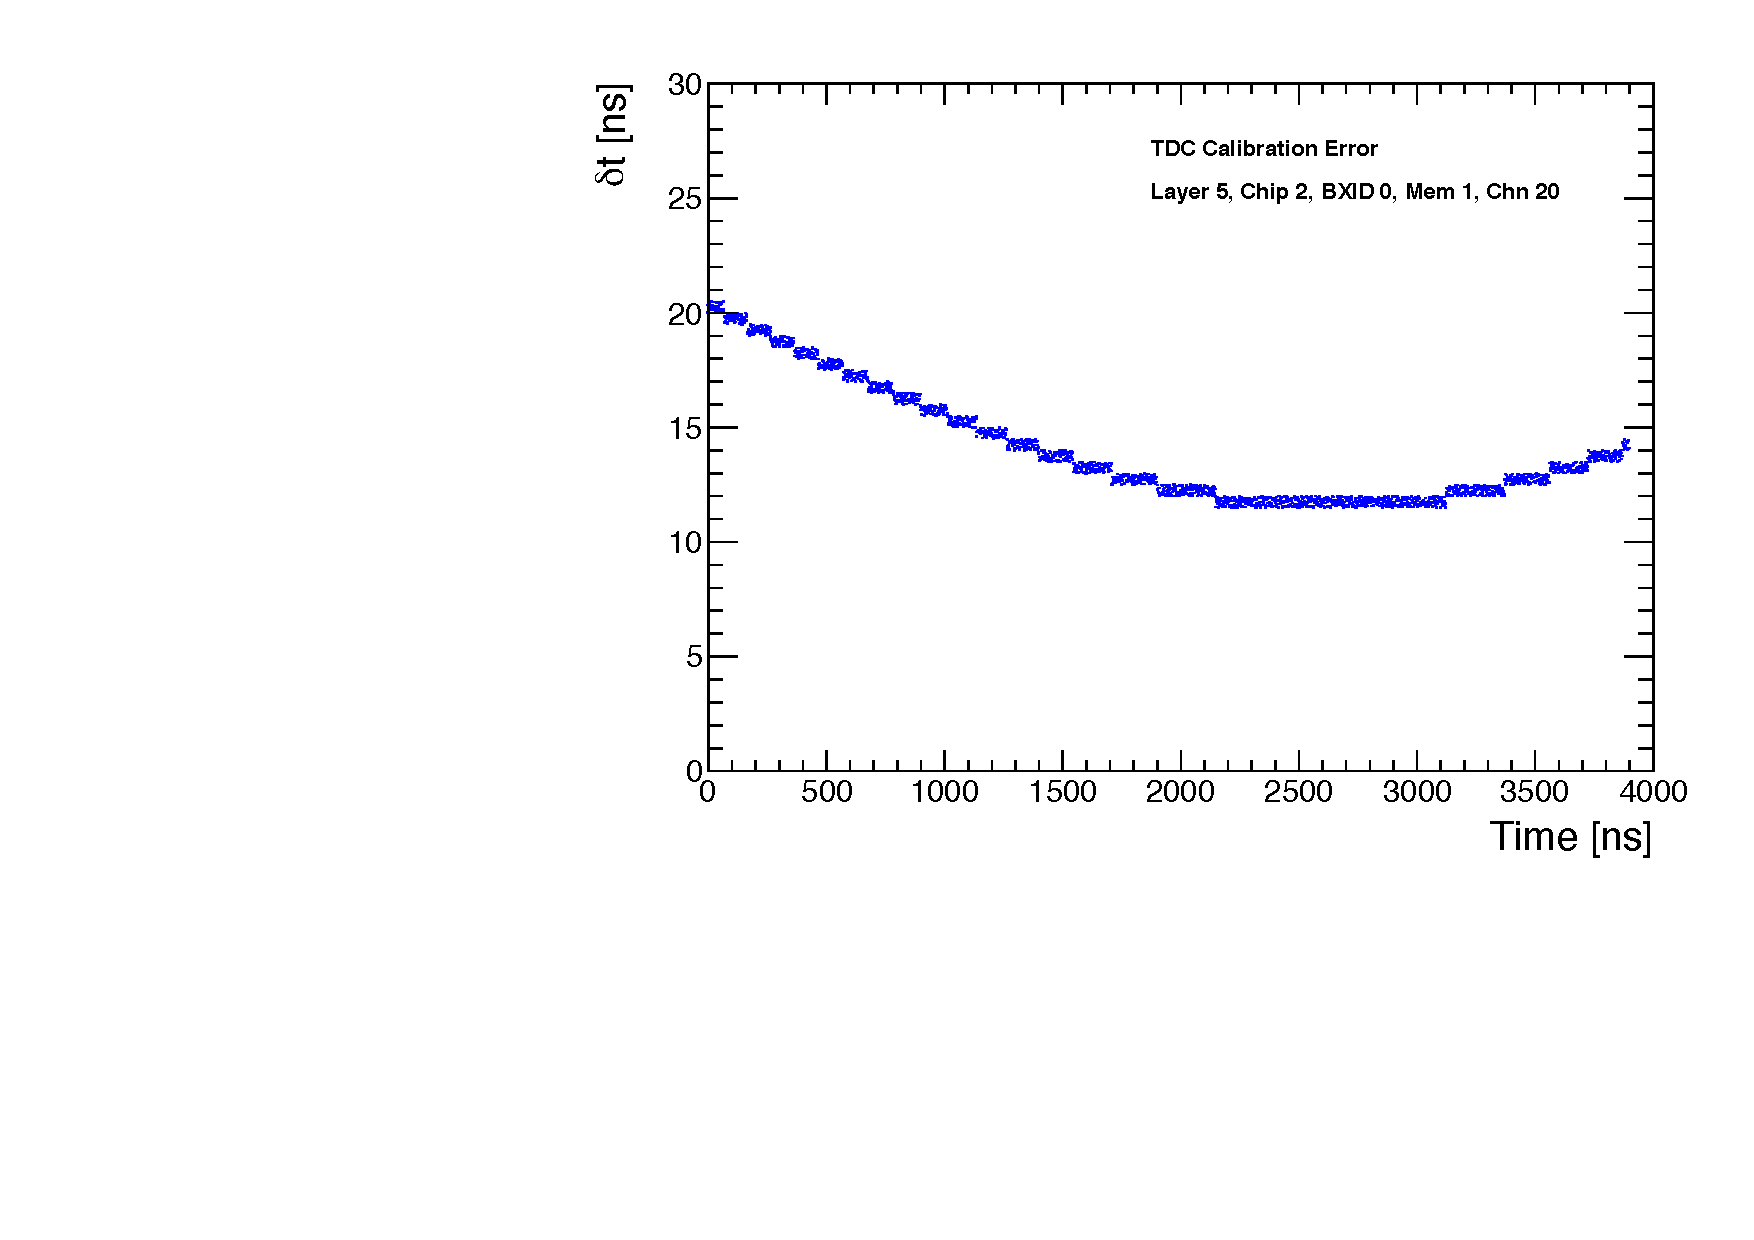
\includegraphics[width=0.5\textwidth]{fig/Muons/TimeErrorEstimation_Layer5.pdf}}
	\caption[]{\textbf{a}: Error distribution made for a single channel on layer 3. The error is variating between 9 and 14 ns but is likely to be over-estimated and not valid for the final time distribution. \textbf{b}: Error distribution made for a single channel on layer 5. The error is variating between 12 and 20 ns but is likely to be over-estimated and not valid for the final time distribution.}
	\label{fig:error_calibration}
\end{figure}

\newpage
\section{Influence of the number of triggered channels and parametrisation in Monte-Carlo.}
\label{appendix:ped_shift}

The correction applied function of the number of hits above 0.5 MIPs is only a global correction not an event to event basis correction. Thus a part of the effect remains in the time distribution or it may be another effect from the electronics that is not yet identified.\\
The effect can be clearly seen in figure \ref{fig:ped_shift_dist_para}. This effect has to be implemented in the simulation in order to match the timing distribution of electrons without also influencing the time distribution for muons. A parametrisation is thus implemented in the Monte-Carlo extracted from data. This parametrisation assumes the following, the effect is additional to the seen muon resolution giving then:
\begin{equation*}
\text{RMS}_{\text{obs}}^2 = \text{RMS}_{\mu}^2 + \text{RMS}_{\text{effect}}^2
\end{equation*}
The $\text{RMS}_{\text{effect}}$ is extracted from data by fitting with a function of the following form:
\begin{equation*}
f(t) = A \times e^{-\frac{(t-\mu_1)^2}{2(\sigma_1^2 + \sigma_{effect}^2)}} + B* \times e^{-\frac{(t-\mu_2)^2}{2(\sigma_2^2 + \sigma_{effect}^2)}} + C
\end{equation*}

\begin{figure}[htbp]
	\subfigure[Time of the first hit distribution for different binning of number of triggered channels in a chip.\label{fig:ped_shift_dist_para}] {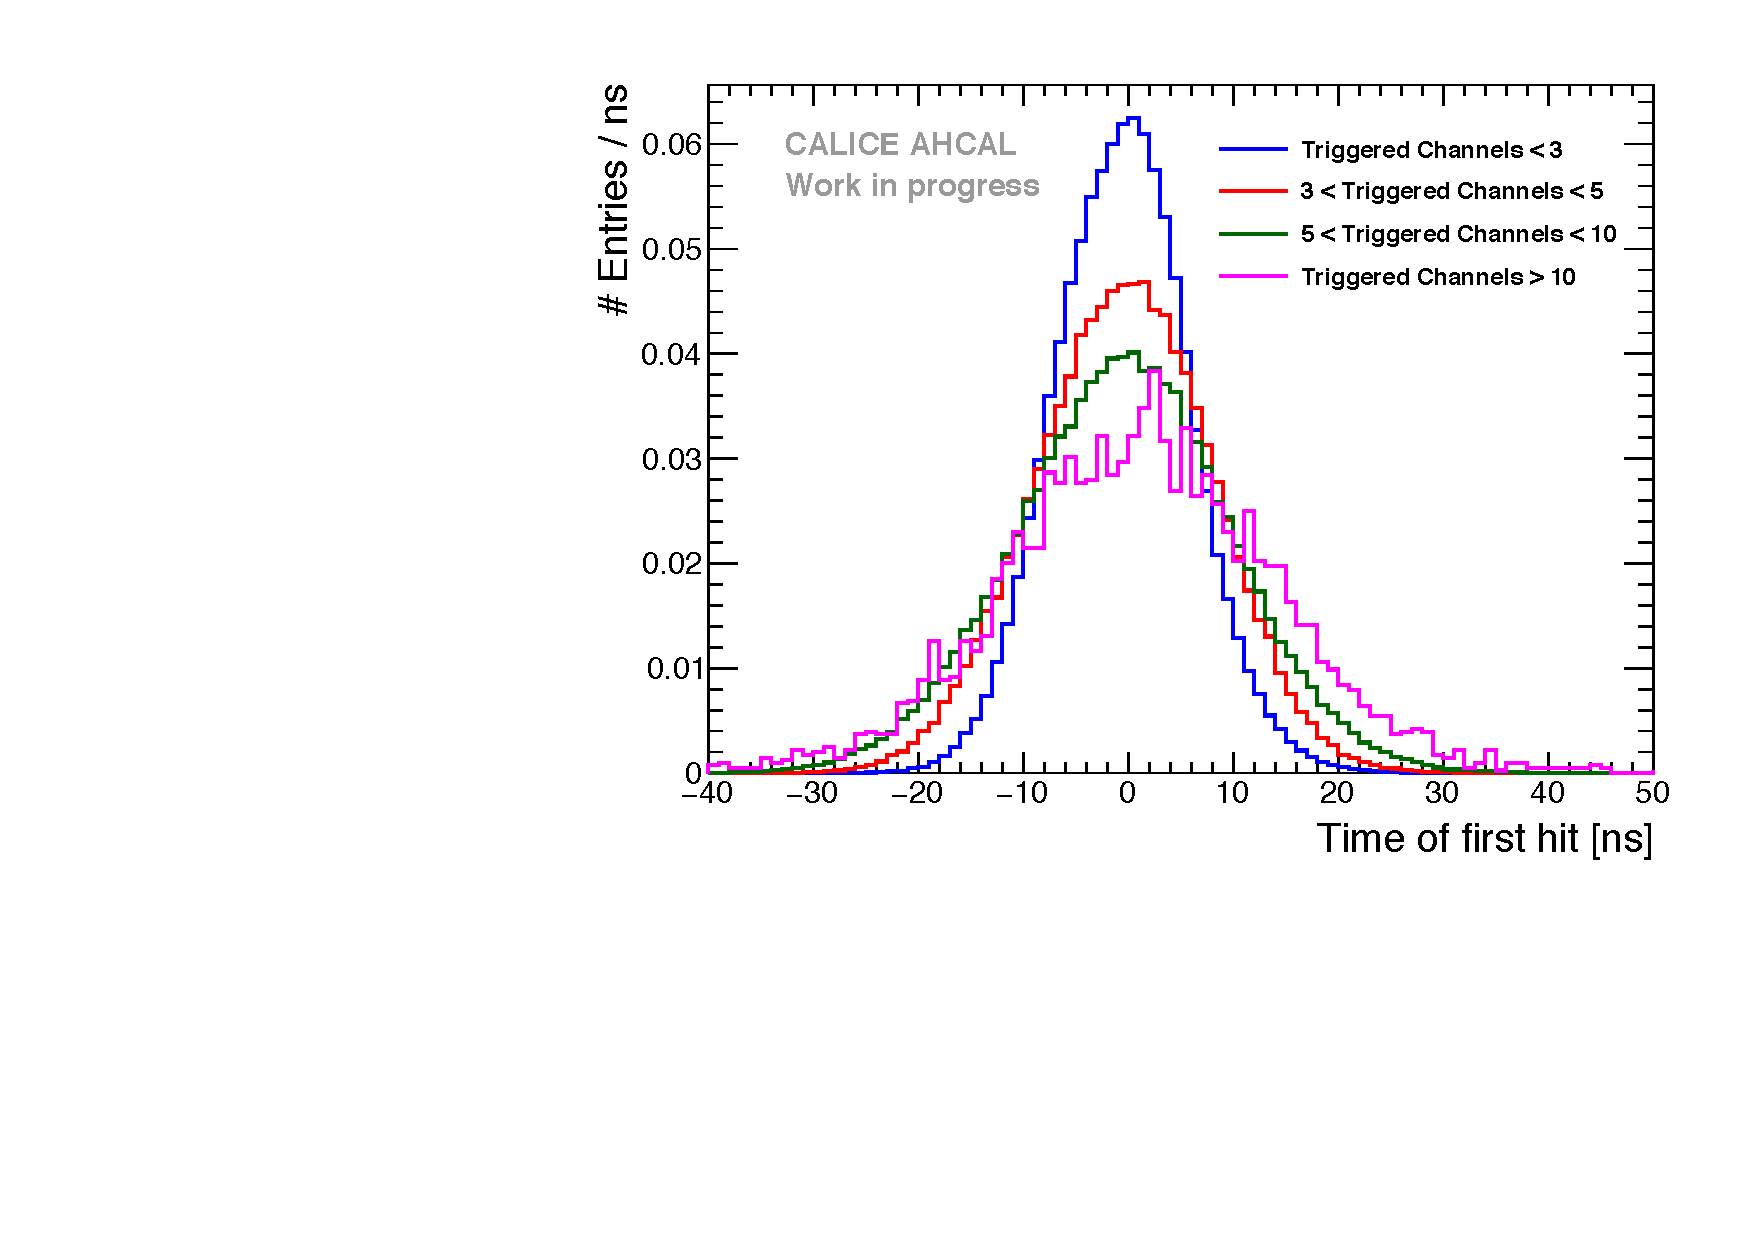
\includegraphics[width=0.5\textwidth]{fig/Electrons/TimingHitsBins_20GeV.pdf}}\hfill
	\subfigure[$\sigma_{effect}$ extracted function of the number of triggered channels in a chip for each energies.\label{fig:para_fit}] {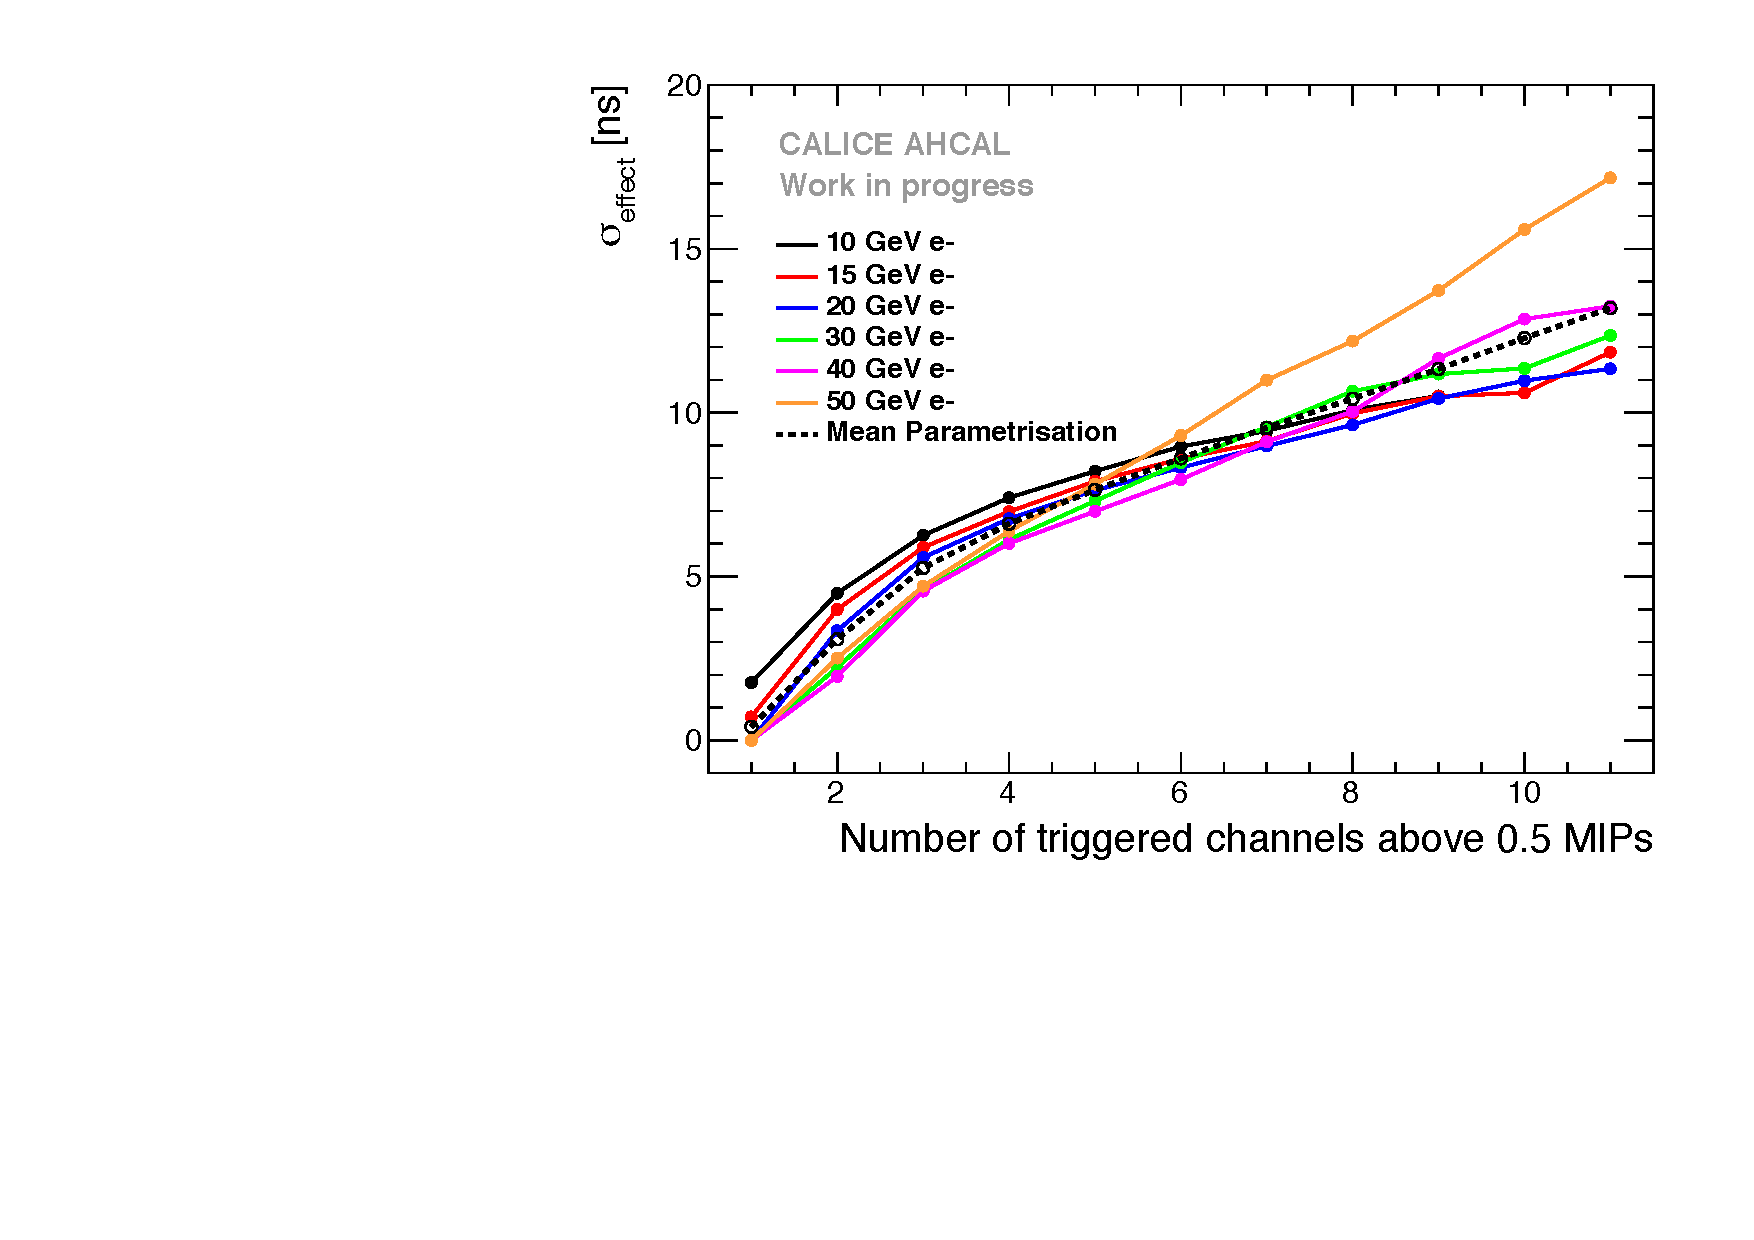
\includegraphics[width=0.5\textwidth]{fig/Electrons/MeanParametrisation.pdf}}
	\caption[]{\textbf{a}: The distribution width is increasing with the number of triggered channels in a chip due to the remaining of the observed effect. \textbf{b}: $\sigma_{effect}$ increases up to 12-15 ns with the number of triggered channels in a chip.}
	\label{fig:mc_para}
\end{figure}

The parameters $\mu_1$, $\sigma_1$, $\mu_2$ and $\sigma_2$ are fixed from table \ref{table:time_res_sim}. By plotting $\sigma_{effect}$ extracted as a function of the number of triggered channels in a chip, one can extract the parametrisation of the effect. This is done for each electron energy point as shown in figure \ref{fig:para_fit}. One can observe that each parametrisation curve is slightly different for each energies. This may be due to the fact that each energy affects not exactly the same part of the detector. To accommodate this, a mean parametrisation is used in Monte-Carlo with the envelope used as uncertainty as shown in figure \ref{fig:mean_para}. Only points up to 10-11 number of channels are extracted from data. Above this, the value of $\sigma_{effect}$ is extrapolated. This should in principle have relatively a small effect for electrons as mainly 6-10 hits are expected per chip. But the effect may be relevant for pions.

\begin{figure}[htbp]
\begin{center}
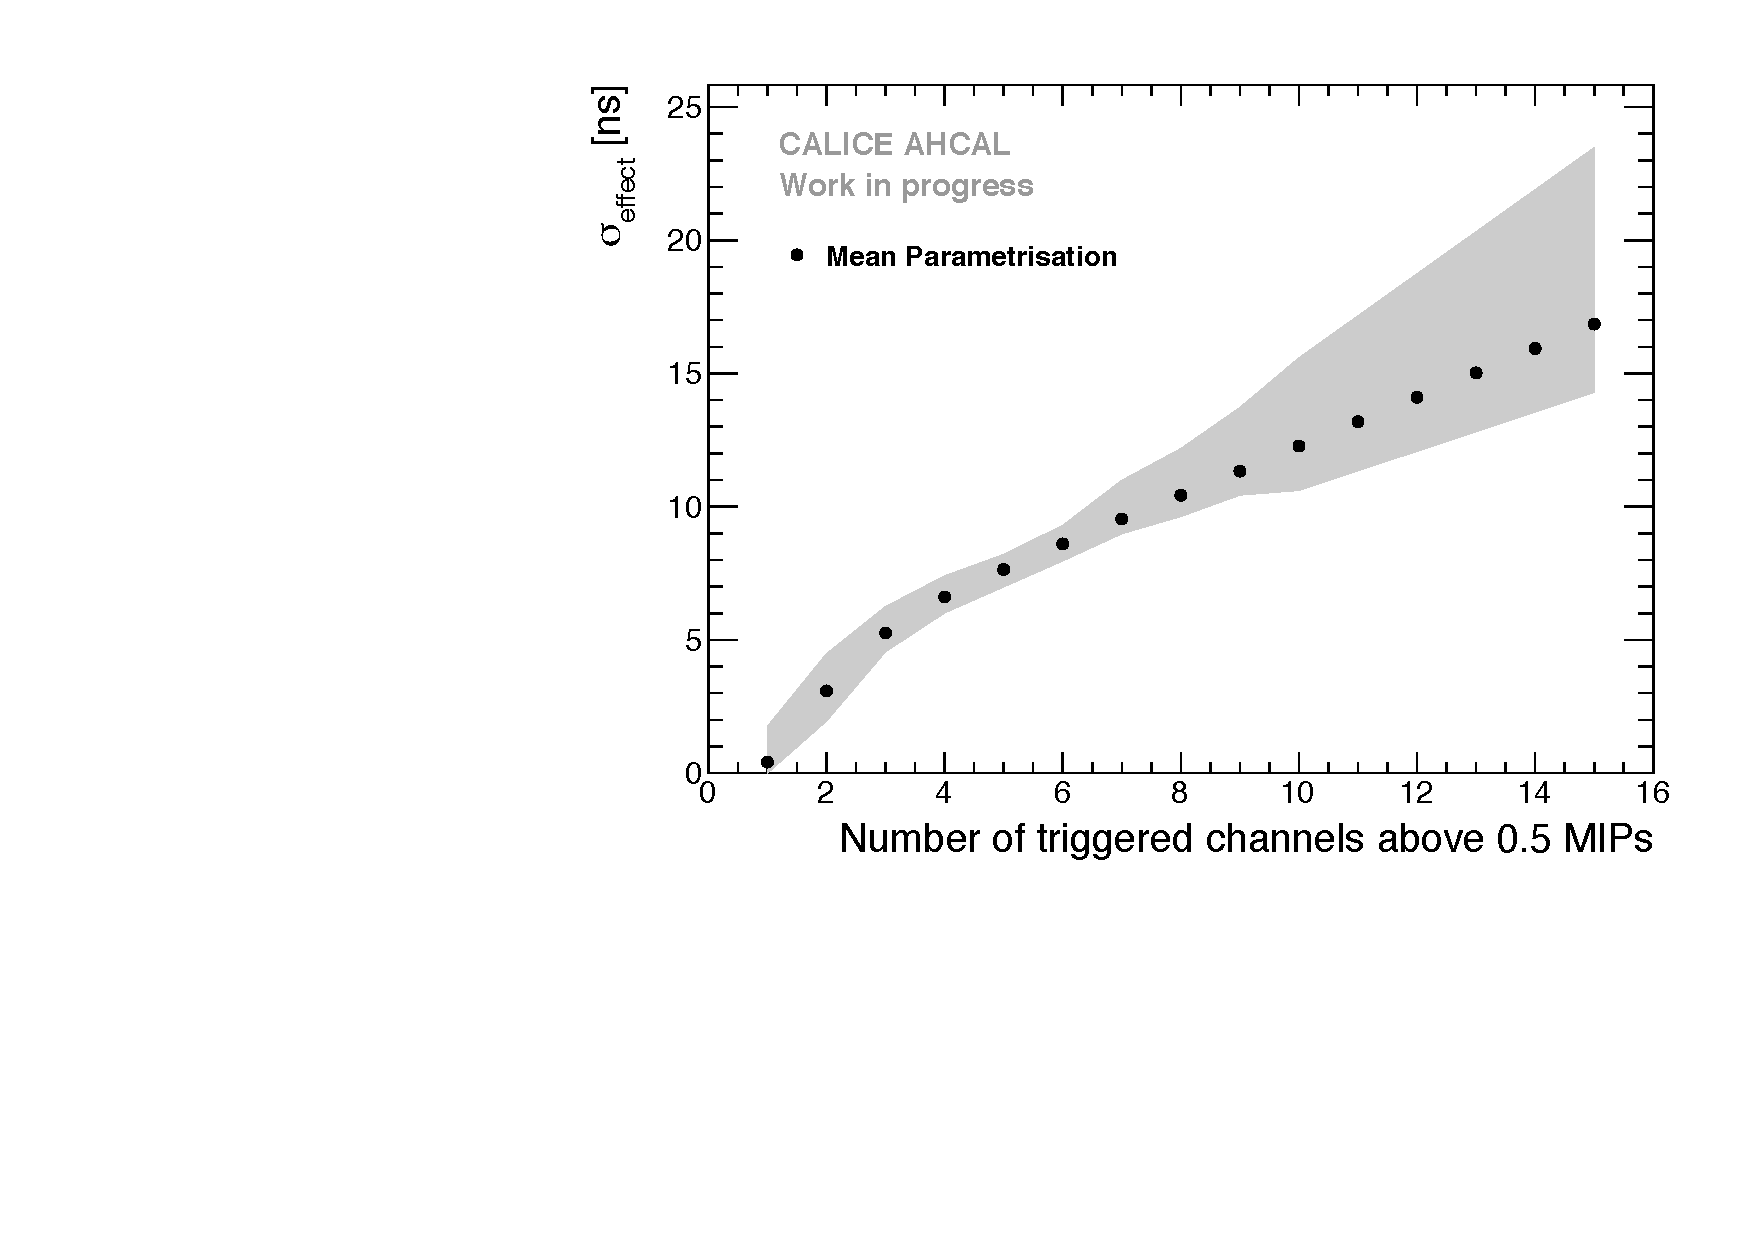
\includegraphics[width=0.6\textwidth]{fig/Electrons/MeanParametrisationWithSystErrors.pdf}
\caption{Mean parametrisation of $\sigma_{effect}$ as a function of number of triggered channels. The grey area represents the uncertainty.}
\label{fig:mean_para}
\end{center}
\end{figure}

\newpage
\section{Noise extraction and effect in timing.}
\label{appendix:noise}

Due to the nature of the detector triggering, noise can't be extracted like the previous CALICE physics prototypes with external triggers between between spills. Moreover if no validation signal is provided by the trigger scintillators, the chip removes noise events stored in memory.\\
One way to avoid this, one can use real events to extract noise. This is can be efficiently done with muon runs as a track in present in the calorimeter due to the muon. By removing the track and keeping remaining hits, noise can be extracted. Muon runs from 24647 to 24656 are used for noise extraction. The events are selected by the cuts shown in table \ref{table:noise_sel}.

\begin{table}[htbp]
\centering
\resizebox{0.9\textwidth}{!}{%
  \begin{tabular}{@{}p{4cm} p{3cm} p{6cm}@{}}
    \hline
    \multicolumn{1}{l}{\textbf{Name}} & \textbf{Beam Energy} & \textbf{Cut}\\
    \hline
    \multirow{3}{*}{Noise selection}& All & $n_{hits}$ in a tower > 7\\& All & 0 < $n_{hits}$ < 30\\& All & $n_{hits}$ in layer < 3\\
    \hline
    \end{tabular}
    }
  \caption{Selection cuts for noise extraction from muon runs.}
  \label{table:noise_sel}
\end{table}

Remaining hits after track removal are considered as noise hit. Initially, the time of these are in TDC values. To get an approximation of the noise distribution, the time of a noise hit is randomly shifted by a flat distribution between 500 and 3500 ns. This acts as a time reference for these hits and thus give a quite good description of the noise time distribution. The figures \ref{fig:noise_energy} and \ref{fig:noise_time} show the energy and time distribution of noise hits.

\begin{figure}[htbp]
	\subfigure[Energy distribution of noise hits.\label{fig:noise_energy}] {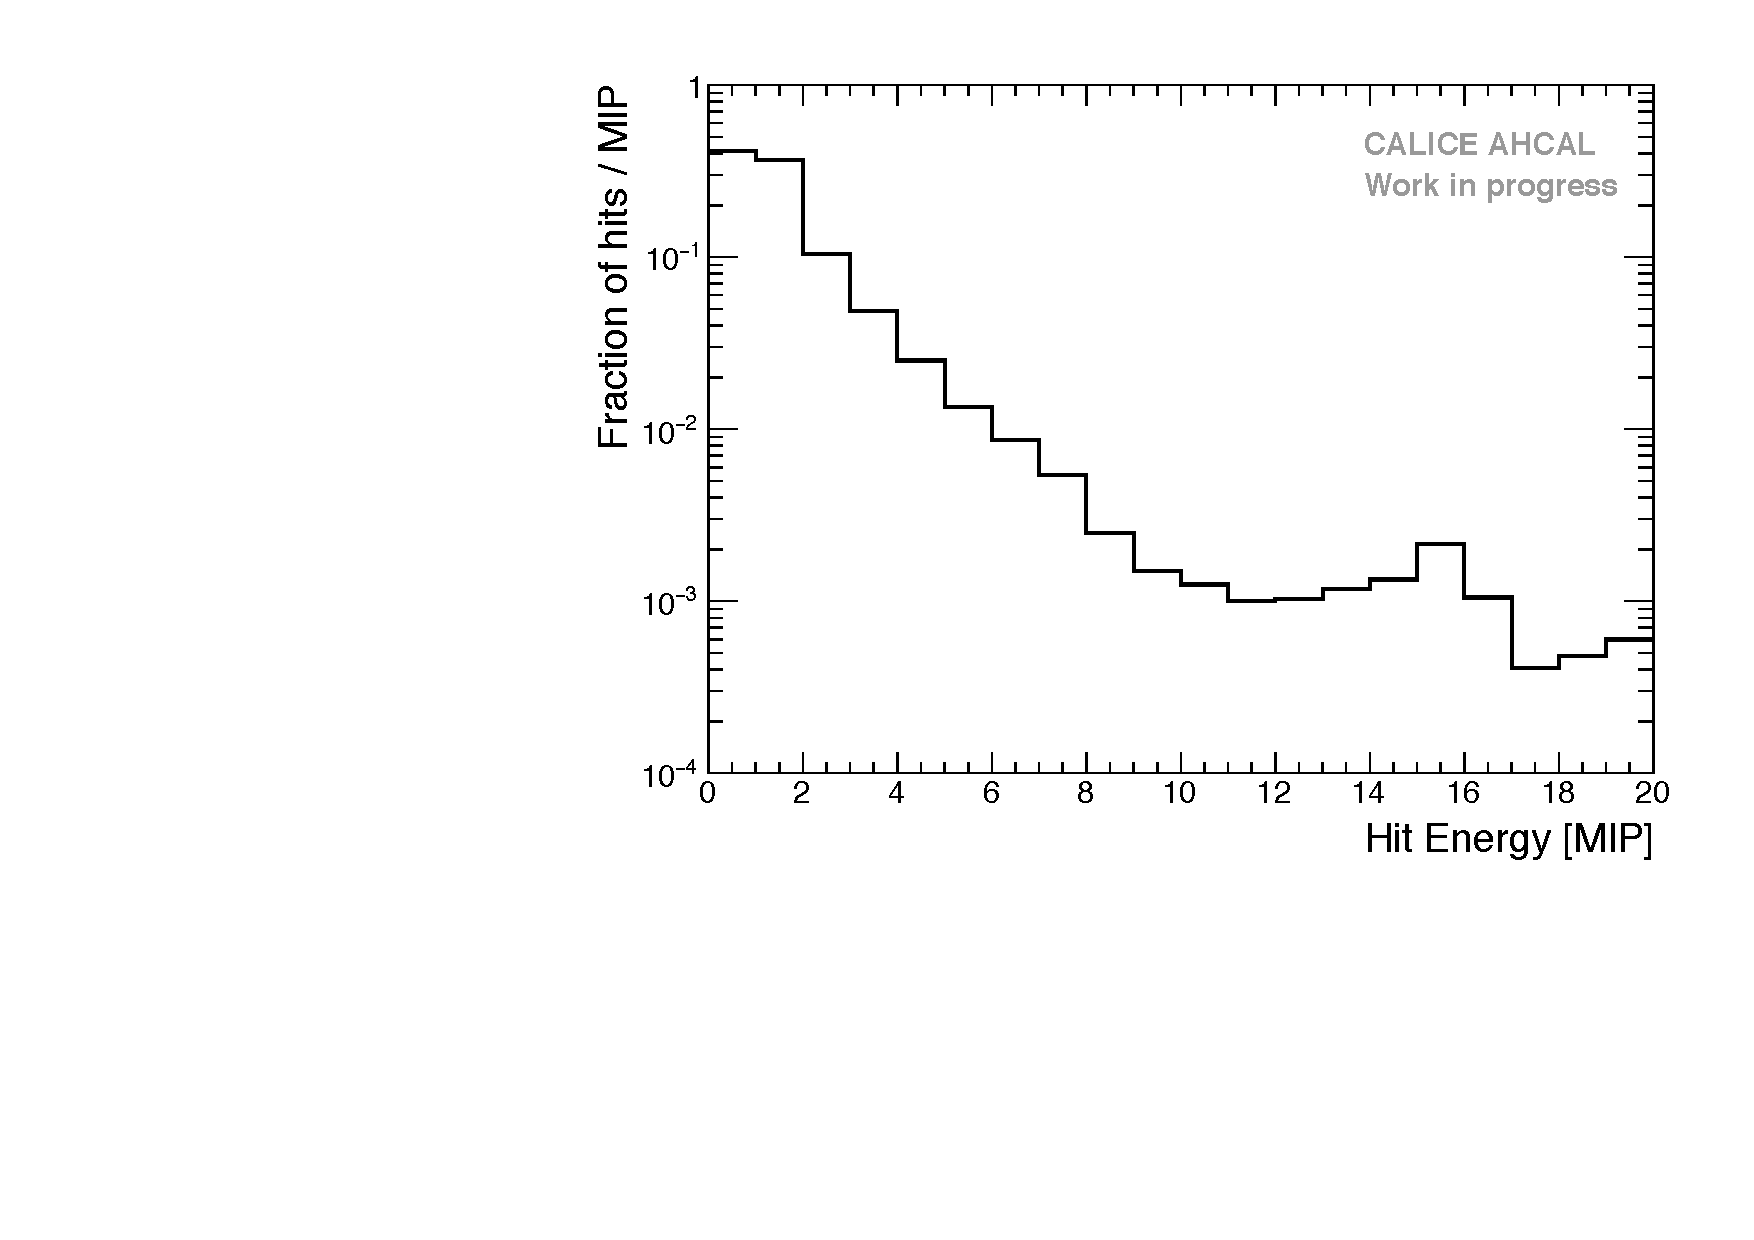
\includegraphics[width=0.5\textwidth]{fig/Muons/Noise_Energy.pdf}}\hfill
	\subfigure[Time distribution of noise hits.\label{fig:noise_time}] {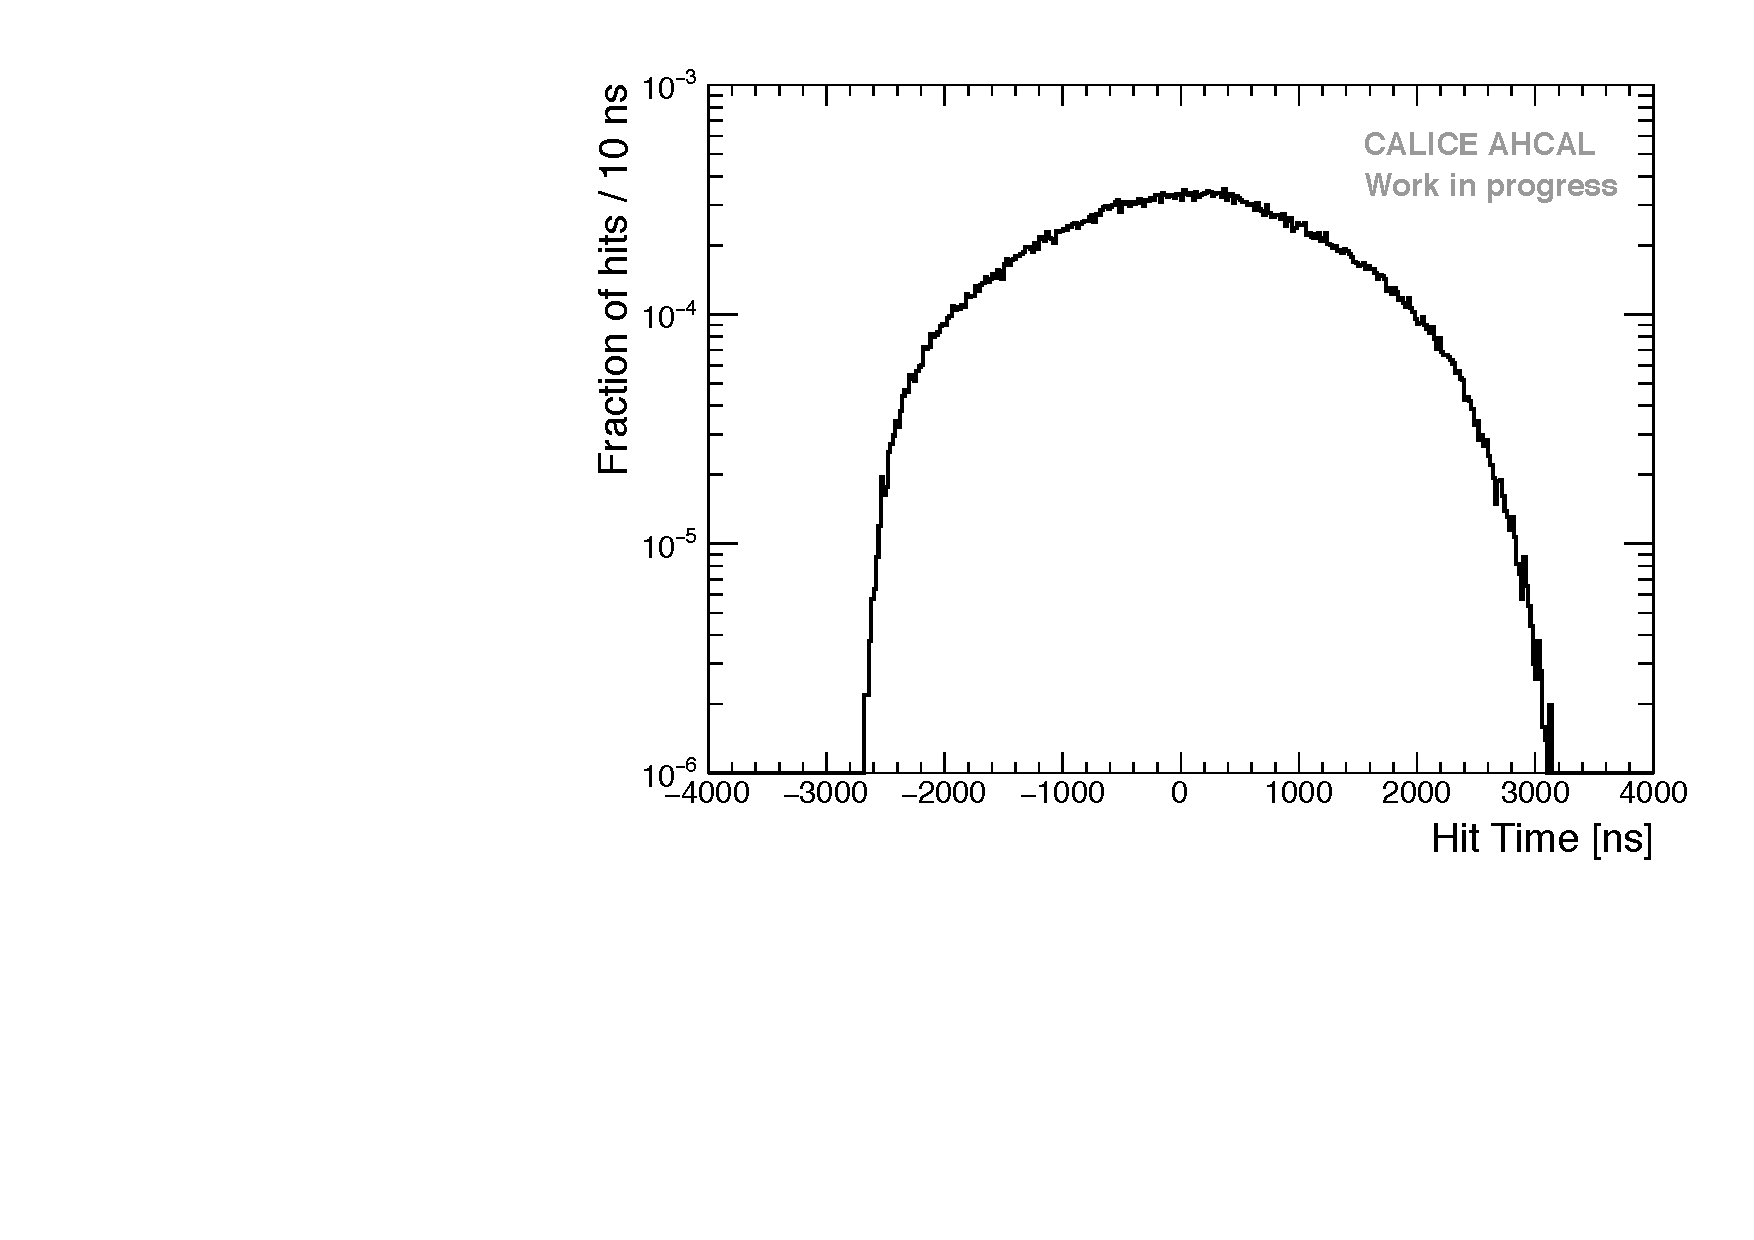
\includegraphics[width=0.5\textwidth]{fig/Muons/Noise_Time.pdf}}
	\caption[]{\textbf{a}: Most of the fraction of noise hits have an energy under 2 MIPs. Higher hit energies may be due to delta electrons from muon tracks but is not expected to have a great impact on timing. \textbf{b}: The shape of the time distribution of noise hits is very important to reproduce well the data in simulation.}
	\label{fig:noise}
\end{figure}

\newpage
\section{Tables of rejected chips.}
\label{appendix:rejection}

\begin{table}[htbp]
\centering
\resizebox{0.9\textwidth}{!}{%
  \begin{tabular}{@{}p{4cm} p{3cm} p{6cm}@{}}
    \hline
    \multicolumn{1}{l}{\textbf{Name}} & \textbf{Beam Energy} & \textbf{Chips}\\
    \hline
    Muon Runs & All & 157, 169-184\\
    \hline
    \end{tabular}
    }
  \caption{Table of chips rejected for muon runs.}
  \label{table:rej_muons}
\end{table}

\begin{table}[htbp]
\centering
\resizebox{0.9\textwidth}{!}{%
  \begin{tabular}{@{}p{4cm} p{3cm} p{6cm}@{}}
    \hline
    \multicolumn{1}{l}{\textbf{Name}} & \textbf{Beam Energy} & \textbf{Chips}\\
    \hline
    Electron Runs & All & 145-150, 151-157, 161-168, 169-184, 188, 191, 197\\
    \hline
    Pion Runs & All & 145-150, 151-157, 161-168, 169-184, 188, 191, 197\\
    \hline
    \end{tabular}
    }
  \caption{Table of chips rejected for electron and pion runs.}
  \label{table:rej_other}
\end{table}

\end{appendix}
